\documentclass[a4paper]{article}
\usepackage[utf8]{inputenc}
\usepackage[usenames,dvipsnames]{color}
\usepackage{ngerman}
\usepackage{textcomp}
\usepackage{longtable}
\usepackage{amssymb}
\usepackage{helvet}
\usepackage{graphicx}
\usepackage{setspace}
\usepackage[super,square]{natbib}
\usepackage[colorlinks=true,linkcolor=black,citecolor=black,urlcolor=blue]{hyperref}
\usepackage[rflt]{floatflt}
\usepackage{geometry}
\usepackage{listings}
\usepackage{fancyhdr}
\geometry{a4paper,left=30mm,right=30mm,top=25mm,bottom=25mm}
% \renewcommand{\rmdefault}{\sfdefault}
\renewcommand{\headrulewidth}{0.0pt}

\newcommand{\cfile}[1]{\texttt{#1}}
\newcommand{\ccaption}[1]{\textsc{#1}}
\newcommand{\cvalue}[1]{\texttt{#1}}
\newcommand{\ckeyword}[1]{\texttt{#1}}

\newcommand{\note}[1]{\textbf{Hinweis:} #1 \par}
\newcommand{\warning}[1]{\textbf{Warnung:} #1 \par}

\newcommand{\rarrow}{\textrightarrow}

\onehalfspacing

\lstset{
    basicstyle=\footnotesize\ttfamily, numbers=left, numberstyle=\footnotesize\ttfamily,
    keywordstyle=\color{blue}\bfseries, commentstyle=\color{Gray}\textit, stringstyle=\color{Maroon},
    stepnumber=1, numbersep=10pt, backgroundcolor=\color{white},
    frame=l, tabsize=2, captionpos=b, breaklines=true, breakatwhitespace=true,
    showspaces=false, showtabs=false, showstringspaces=false,
    title=\lstname, escapeinside={\%*}{*)},
    morekeywords={__file__}
}

\begin{document}

\pagestyle{fancy}
\fancyhf{}
\fancyfoot[R]{\huge{\thepage}}

\vspace*{\fill}
\begin{center}
  \Huge{\textbf{ORCF Custom Content Guide}} \\
  \vspace{2cm}
  \large{Für ORCF \textbf{2011.09p}} \\
  \vspace{1cm}
  \large{\today}
  \vspace{3cm}
\end{center}
\vfill

\newpage

\tableofcontents

\newpage

\section{Custom Content und ORCF}
ORCF wurde von Anfang an darauf ausgelegt, von den Usern um eigene Objekte erweitert zu werden -- mit allen Möglichkeiten, die das Spiel bietet. Dazu ist
diese Anleitung gut, auch wenn die garantiert noch nicht fertig ist, aber hey, das Spiel selbst ist ja auch noch alles andere als fertig und das einzige,
was man bisher erstellen kann, sind einfache Objekte zum Hinstellen. Die können zwar auch animiert sein -- dafür muss man aber etwas programmieren. Auf
die Programmierung wird aber erst in einer zukünftigen Veröffentlichung eingegangen, wenn das System etwas ausgereifter ist.

\subsection{Das Standardpaket}
Alle Objekte, die in dieser Vorabversion enthalten sind, fliegen selbstverständlich raus. Die wurden nur erstellt um grafische Effekte zu demonstrieren
und um etwas rumzuspielen.

Wenn ihr Lust habt, könnt ihr Sets für das so genannte Standardpaket erstellen, damit es standardmäßig bei ORCF mitgeliefert wird. Allerdings gibt es da
neben einigen technischen Anforderungen, die später erwähnt werden, einige Voraussetzungen:
\begin{itemize}
\item
  Die Sets müssen unter einer Creative Commons-Lizenz stehen, die mindestens die unveränderte nichtkommerzielle Weitergabe mit Namensnennung erlaubt,
  vorzugsweise auch noch Veränderungen am Original, damit das Set nicht von den Erstellern selbst an technische Änderungen angepasst werden muss. Ein
  Beispiel ist die Lizenz CC BY-NC-SA 3.0.
\item
  Um darauf hinzuweisen, was erlaubt ist, ist dem Set eine \cfile{readme.txt} beizulegen.
\item
  Sie dürfen demnach keine Inhalte, die nicht unter einer zu der gewählten Creative Commons-Lizenz stehen, enthalten. Das gilt vor Allem für Texturen.
\end{itemize}


\section{Voraussetzungen}

\subsection{Blender}
Das mitgelieferte Export-Script für Objekte funktioniert nur mit Blender 2.5. Ihr benötigt also eine aktuelle Version von Blender sowie grundlegende
Kenntnisse im Umgang mit der Software. Wenn ihr mit Blender 2.4 arbeitet, werdet ihr in 2.5 wahrscheinlich nicht sofort alles an gewohnter Stelle
finden.

\subsection{Das Export-Script}
Im Unterordner \cfile{tools} befindet sich neben zwei ausführbaren Programmen die Datei \cfile{export.py}. Bevor ihr diese zu Blender hinzufügt,
müsst ihr allerdings die Pfade zu einigen ORCF-eigenen Hilfsprogrammen angeben. Wenn ihr die Datei in einem Texteditor öffnet, der Zeilenumbrüche
unterstützt (z.\, B. Kate, Notepad++, \dots ), findet ihr recht weit oben folgende Zeilen:
\begin{lstlisting}[language=python]
ocfgen_exe = '/home/philip/Delphi/orcf/tools/ocfgen'
orcf_data_path = '/home/philip/Delphi/orcf/data/'
orcf_personal_data_path = '/home/philip/orcf-data/'
\end{lstlisting}
Lasst euch nicht von den komischen Namen verwirren, ich schleppe den \cfile{Delphi}-Ordner schon seit gut 5 Jahren mit mir rum, ohne überhaupt noch
Delphi zu benutzen -- ihr müsst einfach die Pfade zu den entsprechenden Zielen angeben.

\subsubsection{Windows}
Unter Windows sieht das beispielsweise so aus:
\begin{lstlisting}[language=python]
ocfgen_exe = 'C:/orcf/tools/ocfgen.exe'
orcf_data_path = 'C:/orcf/data/'
orcf_personal_data_path = 'C:/orcf/data/'
\end{lstlisting}

Beachtet bitte, dass Python auch unter Windows einfache Schrägstriche bei Pfaden akzeptiert und dass die letzten beiden Pfade identisch sein müssen!

\subsubsection{Linux}
Unter Linux liegt der letzte Pfad immer im Userverzeichnis und heißt immer \cfile{orcf-data}. Hier ist also nur der Username zu ändern, während die
anderen beiden Pfade dahin zeigen, wo das Programm liegt -- vorzugsweise in \cfile{/opt/orcf}, wenn es für alle Systembenutzer zugänglich sein soll.


\section{Ordnerstruktur eines Sets}
Objekte liegen \emph{immmer} im \cfile{scenery}-Ordner in einem der Datenordner -- es ist dabei völlig egal, ob es der persönliche Datenordner oder der
Systemordner ist. Unter Windows sind die sowieso gleich. In der ersten Ebene liegen dabei die OCF-Dateien, die auf die einzelnen Objekte im Set
verweisen, sowie die Ordner, in denen die eigentlichen Daten eurer Sets liegen. Damit es nicht zu Überschneidungen kommt, benennt eure Ordner und
OCF-Dateien möglichst nach folgendem Schema:\\
\cfile{Name\_des\_Erstellers-Name\_des\_Sets} für den Ordner und \\
\cfile{Name\_des\_Erstellers-Name\_des\_Sets.ocf} für die OCF-Datei.

Innerhalb des Ordners seid ihr theoretisch völlig frei in der Namensgebung. Es sollten jedoch nur "`normale"' Zeichen verwendet werden, d.\,h.
Buchstaben, Zahlen sowie Unter- und Bindestriche. Leerzeichen führen jedoch zu Problemen.

Weil das Export-Script eine Menge Dateien erzeugt, die durchaus bei verschiedenen Objekten denselben Namen haben können, ist es empfehlenswert, für jedes
Objekt einen eigenen Ordner anzulegen.

\section{Objekte erstellen}
Voraussetzung ist, dass ihr mit Blender modellieren und texturieren könnt. Hier sollen nur die Spezialitäten von Blender im Bezug auf ORCF-Objekte
erläutert werden, nicht aber die Grundlagen, denn das würde zu viel Zeit in Anspruch nehmen -- es gibt mehr als genug gute Blender-Tutorials da draußen.

\subsection{Informationen über das Objekt}
Die meisten Angaben hierzu werden in ORCF selbst angegeben -- der Name des Autors steht allerdings in der Blender-Datei. Um diesen zu setzen, erstellt ihr
im World-Panel ein Custom Property mit dem Namen \ccaption{author} und eurem Namen als Wert:
\begin{center}
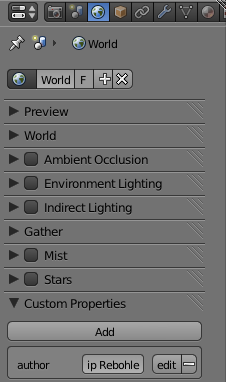
\includegraphics[width=40mm]{../images/blender/world-author.png}
\end{center}
Diese Information wird bei jeder Datei benötigt, also kann es sich durchaus lohnen, ein Template zu erstellen, in dem das bereits drinsteht.

\subsection{Materialien}
Vorweg: Gebt euren Materialien aussagekräftige Namen! Jedes einzelne Material kann im Spiel vom Nutzer verändert werden (v.\,a. die Farbe), da hilft
es wenig, wenn das Material "`Material.005"' heißt. Leerzeichen sorgen aber für Probleme bei der OCF-Dateierstellung, verwendet also statt Leerzeichen
bitte Unterstriche. Umlaute sind auch verboten, weil Windows Umlaute anders codiert als andere Systeme -- hier gilt also dasselbe wie schon bei der
Benennung der Dateien weiter oben.

\warning{Nutzt Transparenz bitte nur, wenn nötig (z.\,B. bei Fenstern), denn das Rendering von transparenten Objekten ist in ORCF schlecht implementiert
  und führt zu Anzeigeproblemen.}

\subsubsection{Benutzbare Eigenschaften}
\begin{itemize}
\item Materialfarbe (\ccaption{Diffuse}, \ccaption{Diffuse \rarrow Intensity}). Kann vom Spieler geändert werden.
\item Emission (\ccaption{Shading \rarrow Emit}). Aktiv für selbstleuchtende Materialien. Kann vom Spieler geändert werden.
\item Glanzlicht-Intensität (\ccaption{Specular \rarrow Intensity})
\item Glanzlicht-Härte (\ccaption{Specular \rarrow Hardness})
\item Durchsichtigkeit (\ccaption{Transparency \rarrow Alpha})
\item Reflexionsstärke (\ccaption{Mirror \rarrow Reflectivity})
\item Reflexionsmodus (\ccaption{Mirror \rarrow Max Distance}). Ein Wert von \cvalue{0} bedeutet, dass \emph{immer} eine fast statische Environment Map
  auf das Objekt gelegt wird (empfehlenswert bei Objekten mit geringer Reflexionsstärke sowie sehr großen Objekten), jeder größere Wert bedeutet, dass
  die Reflexionstextur dynamisch gerendert wird, wenn der User dies in den Grafikeinstellungen aktiviert hat
\item Texturen, dazu aber mehr im Abschnitt \ref{objects_textures} Texturen.
\end{itemize}

\subsubsection{Custom Properties}
\begin{itemize}
\item \ccaption{displacementHeight} -- betrifft nur User mit aktiviertem Parallax Occlusion Mapping. Gibt die maximal simulierte Tiefe in Metern an,
      Standardwert ist \cvalue{0.04}, Werte bis \cvalue{0.20} erzeugen in der Regel gute Ergebnisse.
\end{itemize}

\subsection{Texturen}
\label{objects_textures}
ORCF kann zwei verschiedene Typen von Texturen verarbeiten: Farbtexturen und Bump Maps. Bump Maps sind Texturen, die Informationen über die Ausrichtung
und die Verschiebung von der Oberfläche eines Objekts enthalten, um den Detailgrad ohne zusätzliche Polygone deutlich zu erhöhen. Die Erstellung von
Bump Maps mit Blender wird im Abschitt \ref{bumpmaps} Bumpmaps erläutert.
\note{Bitte sorgt dafür, dass eure Farbtexturen nur dann einen Alphakanal haben, wenn er wirklich genutzt wird! Sonst funktionieren Dinge wie Parallax
  Occlusion Mapping nicht und es kommt zu unschönen Artefakten.

\subsubsection{Benutzbare Eigenschaften}
\begin{itemize}
\item Typ muss \cvalue{Image or Movie} sein
\item \ccaption{Image \rarrow Source} muss auf eine TGA-Datei verweisen
\item \ccaption{Mapping \rarrow Coordinates} muss auf \cvalue{UV} stehen
\item bei \ccaption{Influence} kann entweder \cvalue{Color} oder \cvalue{Normal} aktiviert werden. Wenn \cvalue{Color} aktiv ist, so wird die Farbe
  der Textur im Spiel mit der gewählten Materialfarbe multipliziert -- wenn euer Objekt also einfärbbar sein soll, achtet darauf, dass eure Textur
  möglichst nur Grautöne beinhaltet. Wenn \cvalue{Normal} aktiv ist, handelt es sich um eine Bumpmap.
\end{itemize}

\subsection{Objekte}
Das, was in ORCF als Mesh bezeichnet wird, heißt in Blender "`Object"' und stellt die Geometrie dar.

\subsubsection{Benutzbare Eigenschaften}
\begin{itemize}
\item Position (\ccaption{Transform \rarrow Location}). Ergibt sich, wenn man im Object Mode das Objekt verschiebt.
\item Drehung (\ccaption{Transform \rarrow Rotation}). Ergibt sich, wenn man im Object Mode das Objekt dreht.
\item Elternobjekt (\ccaption(Relation \rarrow Parent}). Alle Transformationsoperationen des Elternobjekts werden auch auf dieses Objekt übertragen,
  besonders bei Animationen interessannt.
\end{itemize}
\warning{Die Skalierung (\ccaption{Transform \rarrow Scale}) kann \emph{nicht} benutzt werden! Wenn ihr skaliert, tut dies \emph{immer} im Edit Mode.}

\subsubsection{Custom Properties}
\begin{itemize}
\item \ccaption{min\_dist} -- falls mehrere LODs benutzt werden, gibt dies die minimale Distanz an, die das Objekt zum Betrachter haben muss, um an-
  gezeigt zu werden. Wenn keine LODs benutzt werden oder das Objekt den höchstmöglichen Detailgrad besitzt, sollte diese Eigenschaft nicht benutzt
  werden.
\item \ccaption{max\_dist} -- falls mehrere LODs benutzt werden, gibt dies die maximale Distanz an, die das Objekt zum Betrachter haben muss, um an-
  gezeigt zu werden. Wenn keine LODs benutzt werden oder das Objekt den niedrigsten Detailgrad besitzt, sollte diese Eigenschaft nicht benutzt
  werden.
\end{itemize}

\subsection{Lampen}
Vorweg: Um eine Lampe in ORCF verwenden zu können, muss sie als Parent ein Objekt haben. Außerdem hat ORCF ein ähnliches Beleuchtungsmodell wie
Blender, die genauen Berechnungen sind aber doch anders, deswegen sehen die Ergebnisse beim Rendern nicht zwangsläufig gleich aus.

\subsubsection{Benutzbare Eigenschaften}
\begin{itemize}
\item Position -- ergibt sich, wenn die Lampe verschoben wird.
\item Typ muss \cvalue{Point} sein
\item Schatten (\ccaption{Shadow}) muss auf \cvalue{Ray Shadow} gesetzt werden, wenn die Lampe Schatten werfen soll.
\item Farbe (\ccaption{Lamp}) -- wird in zukünftigen ORCF-Versionen auch vom Spieler geändert werden können. Erstellt daher bitte nicht für verschiedene
  Beleuchtungsfarben eigene Objekte.
\item Energie (\ccaption{Lamp \rarrow Energy}) -- wird ebenfalls eines Tages vom Spieler geändert werden können.
\item Leuchtweite (\ccaption{Lamp \rarrow Energy}) -- gibt an, in welcher Entfernung die Lampe nur noch die Hälfte ihrer ursprünglichen Leuchtkraft
  besitzt. Wird ebenfalls eines Tages vom Spieler geändert werden können.
\end{itemize}

\subsubsection{Custom Properties}
\begin{itemize}
\item \ccaption{onlyNight} -- der Wert spielt hier keine Rolle, wenn die Eigenschaft gesetzt ist, leuchtet die Lampe nur bei Nacht.
\end{itemize}

\section{Linken von externen Ressourcen}
Ihr könnt, um eine Menge Ressourcen zu sparen, Materialien und vor Allem Texturen aus vorher erstellten Blender-Dateien einbinden. Dazu geht ihr
im \ccaption{File}-Menü auf \ccaption{Link}, wählt die Datei aus und sucht dort das entsprechende Material oder die entsprechende Textur. Diese lassen
sich dann auf herkömmliche Weise auswählen, als wären sie in die Datei integriert.

Das sorgt dafür, dass die gelinkten Daten nicht mit in die OCF-Datei geschrieben werden und auch im Spiel nicht mehrfach geladen werden. Das spart
Speicherplatz auf der Festplatte und auf der Grafikkarte, und gerade da sollte man sehr sparsam sein. Diese Funktionalität entspricht etwa
den aus RCT3 bekannten Shared Textures. Nicht möglich ist das allerdings bei Objekten, die Geometrie muss also jedes mal mit exportiert werden.

\section{Bumpmaps erstellen mit Blender}
\label{bumpmaps}
Hier soll kurz erklärt werden, wie man mit Blender eine Bumpmapaus einem Objekt erstellt.

\subsection{Das Objekt}
Das Objekt wird nicht ins Spiel importiert. Es dient lediglich dazu, Polygone in den eigentlichen Objekten einzusparen, ohne jedoch an Detailreichtum
einzubüßen -- daher muss hier bei diesem Objekt keine Rücksicht auf die Anzahl der Polygone genommen werden. Im Grunde erstellt ihr hier genau das, was
ihr ansonsten in das Objekt mit eingebaut hättet, beispielsweise Dachziegel.

\subsection{Das Material}
Ihr weist dem Objekt allerdings nicht die Farben zu, die das Objekt, das die Bumpmap nutzt, später haben soll. Der Trick liegt darin, das Objekt ohne
Farben und ohne Beleuchtung zu rendern. Dazu färbt ihr das Material schwarz und aktiviert \ccaption{Shading \rarrow Shadeless}, außerdem muss für die
Höheninformationen noch \ccaption{Transparency} aktiviert und der Modus auf \cvalue{Mask} gestellt werden.
\begin{center}
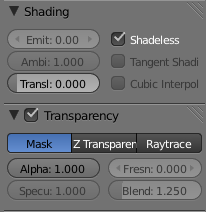
\includegraphics[width=40mm]{../images/blender/bumpmap-material.png}
\end{center}

\subsection{Die Normalentexturen}
Hier liegt eigentlich das Geheimnis. Blender kann mit einigen Tricks die Normale als Farbinformationen auf das Material legen. Dazu müsst ihr verstehen,
wie eine Bumpmap eigentlich aussieht:

Jeder Pixel auf der Bumpmap repräsentiert einen Normalenvektor aus den Komponenten X, Y und Z. Die Werte liegen dabei alle zwischen -1 bis 1 -- auf der
Textur werden sie durch rote, grüne und blaue Farbkomponenten mit einem Wertebereich von 0 bis 255 dargestellt. Zunächst erstellt ihr also eine Textur
für die Z-Komponente der Normale. Die ist blau und muss genau dieselben Eigenschaften haben wie unten dargestellt:

\begin{center}
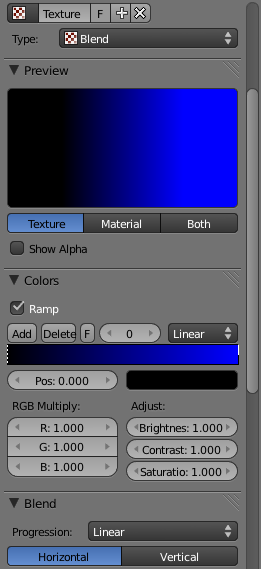
\includegraphics[width=40mm]{../images/blender/bumpmap-texture-1.png}
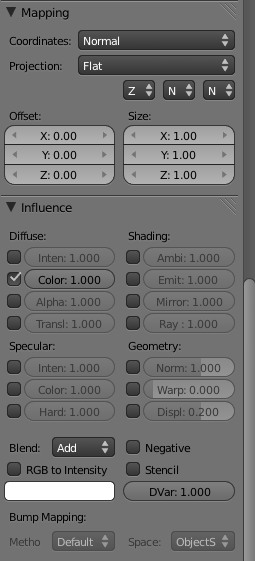
\includegraphics[width=40mm]{../images/blender/bumpmap-texture-2.png}
\end{center}

Wichtig ist, dass das Blau ein reines und volles Blau ist, also keine anderen Farbanteile mehr vorhanden sind.

Am Wichtigsten ist hier die Einstellung \ccaption{Mapping \rarrow Coordinates}. Mit dem Wert \cvalue{Normal} wird Blender angewiesen, die Normalen als
Quelle für das Texturmapping zu verwenden.

Unter \ccaption{Mapping \rarrow Projection} finden sich 3 Auswahlboxen. Die erste davon steht auf \cvalue{Z}, die anderen beiden auf \cvalue{N}. Damit
teilen wir der Blender mit, dass nur der Z-Anteil der Normale berücksichtigt werden soll.

Achtet aber auch darauf, bei \ccaption{Influence \rarrow Blend} \cvalue{Add} auszuwählen, denn sonst seht ihr immer nur eine der drei Texturen.

Ihr müsst jetzt noch zwei weitere Texturen erstellen, eine rote für die X-Anteile und eine grüne für die Y-Anteile. Dazu muss lediglich die Farbe
geändert werden und das Mapping ist von \cvalue{Z} auf \cvalue{X} bzw. \cvalue{Y} zu stellen.

Am Ende sollte die Materialvorschau etwa folgendes ausspucken:

\begin{center}
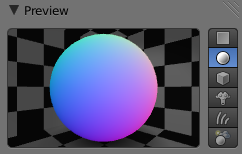
\includegraphics[width=40mm]{../images/blender/bumpmap-material-preview.png}
\end{center}

\subsection{Die Höhentextur}
Damit Parallax Occlusion Mapping mit dieser Bumpmap funktioniert, müsst ihr noch eine Alphatextur erstellen. Die ist sehr ähnlich zu den Normalentexturen,
allerdings mit den folgenden Unterschieden:
\begin{itemize}
\item Die Textur geht nicht von Schwarz zu einer Farbe, sondern von voll durchsichtig zu weiß.
\item Das Mapping benutzt nicht die Z-Komponente der Normale, sondern die Z-Position im World Space (dazu die Einstellung \cvalue{Global} bei \ccaption{Mapping \rarrow Coordinates}.
\end{itemize}

Alles in Allem sollte das etwa so aussehen:

\begin{center}
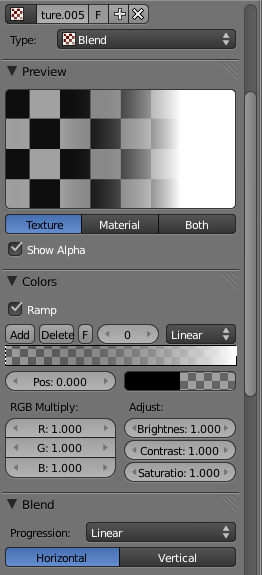
\includegraphics[width=40mm]{../images/blender/bumpmap-texture-3.png}
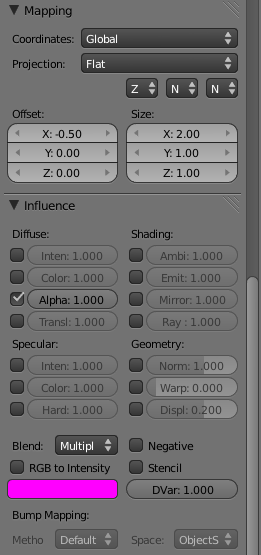
\includegraphics[width=40mm]{../images/blender/bumpmap-texture-4.png}
\end{center}

Offset und Size sind dabei so gewählt, dass für ein Objekt, dessen Z-Werte zwischen 0 und 1 liegen, eine perfekte Alpha-Map erstellt wird. Für andere
Wertebereiche müsst ihr gegebenenfalls etwas rumexperimentieren, oft ist es aber am einfachsten, das Objekt an die richtige Stelle in der Welt zu
verschieben und zu skalieren. Skaliert euer Objekt aber keinesfalls ausschließlich in Z-Richtung, denn dadurch würden die Normalen verfälscht!

\subsection{Die Kamera}
Erstellt eine neue Kamera und setzt diese über das Objekt. Wie hoch sie liegt, ist egal, da sie nicht perspektivisch ist, sondern orthogonal. Das sollte
dann etwa so aussehen:

\begin{center}
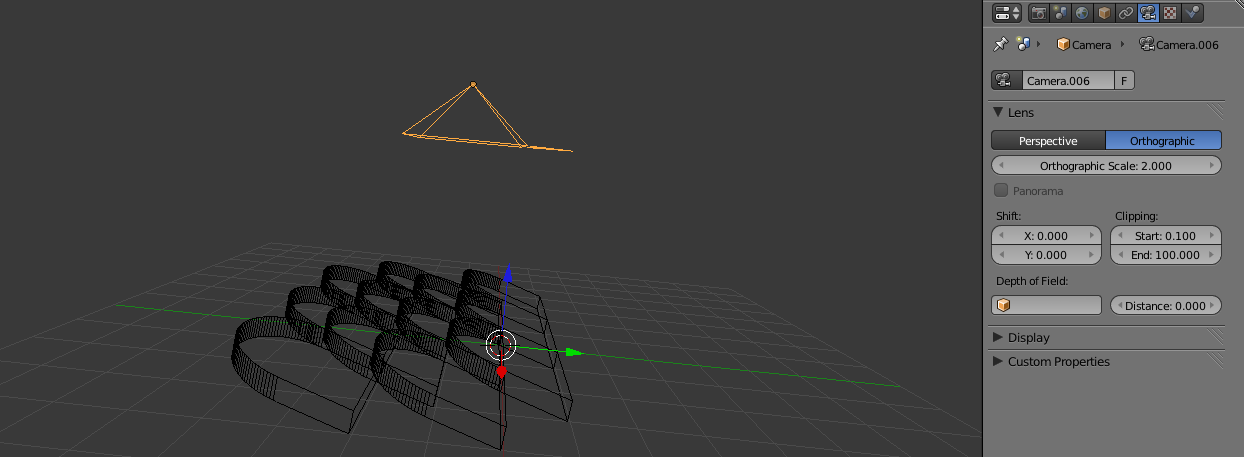
\includegraphics[width=150mm]{../images/blender/bumpmap-camera.png}
\end{center}

Im Scene-Panel könnt ihr die neue Kamera dann als Standardkamera festlegen, das ist unter Anderem für Rendervorgänge nötig.

Wie ihr \ccaption{Orthographic Scale} wählt, hängt letztenendes von euerm Objekt ab. Von der Kamera aus sollte das gesamte Objekt sichtbar sein,
ggf. ist es aber nötig, dass nur ein Teil sichtbar ist, damit die Textur kachelbar bleibt, wie hier im Beispiel mit den Dachziegeln.

\subsection{Rendereinstellungen}
Damit die Bumpmap auch unverfälscht auf den Bildschirm gebracht wird, müsst ihr zunächst Blenders Farbkorrekturen abstellen und RGBA-Rendering aktivieren.
Das geht mit den folgenden Einstellungen im Render-Panel:

\begin{center}
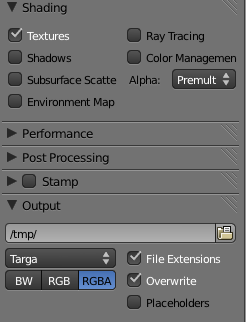
\includegraphics[width=40mm]{../images/blender/bumpmap-render.png}
\end{center}

Wählt außerdem eine passende Größe, oftmals sind Bumpmaps von 256x256 Pixeln Größe völlig ausreichend.

\subsection{Und.. Rendern!}
Nun sind alle Einstellungen getan und ihr könnt die Bumpmap rendern. Bei den Dachziegeln sieht diese etwa so aus, wenn man in Blenders Bildansicht
die Alphakanaldarstellung aktiviert:

\begin{center}
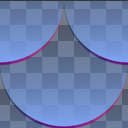
\includegraphics[width=40mm]{../images/blender/bumpmap.png}
\end{center}

Und das Ganze dann im Spiel:
\begin{center}
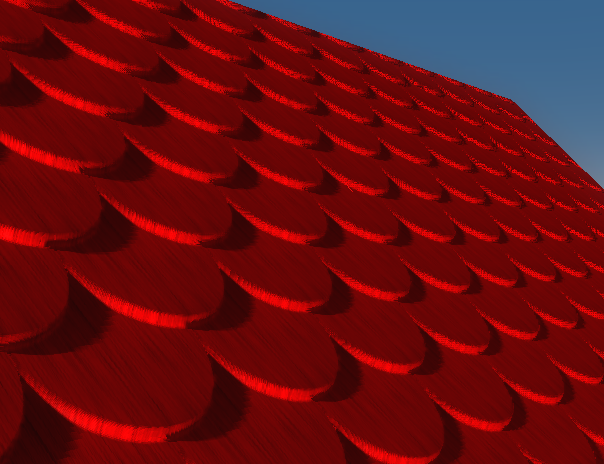
\includegraphics[width=40mm]{../images/blender/bumpmap-ingame.png}
\end{center}

\section{Exportieren}
Im Normalfall genügt ein Klick auf den entsprechenden Menüeintrag:

\begin{center}
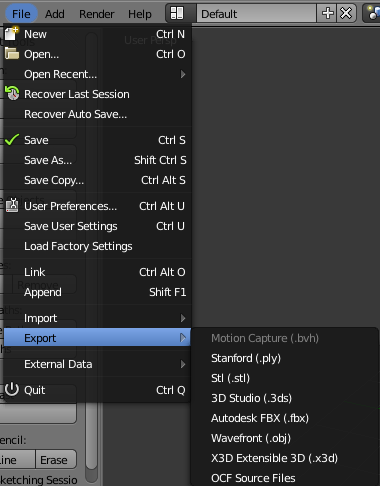
\includegraphics[width=60mm]{../images/blender/blender-menu.png}
\end{center}

Solltet ihr eine Fehlermeldung erhalten, probiert folgendes:
\begin{itemize}
\item Speichert die Datei und ladet sie einmal neu. Das sorgt dafür, dass unbenutzte Ressourcen wirklich gelöscht werden, und somit den Exporter nicht
  weiter stören.
\item Wenn das nichts hilft, öffnet in Blender eine Pythonkonsole und gebt folgendes ein:
  \begin{lstlisting}[language=python]
  bpy.ops.export_scene.ocf("/da/wo/eure/Blenderdatei/liegt/")
  \end{lstlisting}
  und schaut auf die Ausgabe. Die Meldung kann auf fehlerhafte Eingaben zurückzuführen sein, aber auch auf einen Bug im Script.
\item Sollte das Script durchlaufen, aber keine OCF-Datei in dem Ordner, wo auch eure Blenderdatei ist, auftauchen, so liegt das Problem bei der finalen
  Erstellung der OCF-Datei aus den Einzeldateien. Öffnet eine Kommandozeile in dem Ordner, in dem eure Blender-Datei liegt und führt die
  \cfile{.bat}-Datei (Windows) bzw. die \cfile{.sh}-Datei (Linux, Mac OS X) aus, die sich in dem Ordner befindet. Fehler dieser Art sind oft auf
  fehlerhafte Benennungen von jeglichen Objekten in Blender zurückzuführen, besonders Leerzeichen und Umlaute sorgen hier für Probleme, aber es kann
  genau so gut auch an einem Bug liegen.
\end{itemize}

\end{document}